\begin{frame}[fragile]{Why Finite Automata Are Not Enough}

    \begin{itemize}
        \item $L=\{a^{n}b^{n} \mid n \geq 1\}$ cannot be described by a FA.
        \item For a rejected word like \texttt{aaaabb},
        standard parsers identify the error at the end.
        %\item Standard parsers fail at the end of the input, obscuring the actual root cause (the extra bracket):
    \end{itemize}
    
    \vspace{0.4cm}

    \begin{columns}[T] % The [T] aligns the columns at the top
        
        % Left Column: C Code
        \begin{column}{0.46\textwidth}
            \textbf{Source Code:}
\begin{lstlisting}[language=C, basicstyle=\ttfamily\scriptsize, frame=single]
int main(){
    for(int i=0; i<10; i++){{ // Error
        printf("hello");
    }
}
\end{lstlisting}
        \end{column}

        % Right Column: Compiler Error
        \begin{column}{0.52\textwidth}
            \textbf{Parser Output:}
            % Note: Keep the verbatim text flush left so it doesn't add weird spaces
\begin{small}
\begin{verbatim}
error: expected '}' at end of input
5 | }
  | ^
\end{verbatim}
\end{small}
        \end{column}

    \end{columns}

\end{frame}

\section{Current Research: Explaining CFGs}

\begin{frame}{Fragility of Acceptance vs. Robustness of Rejection}
    In Context-Free Languages, consider the balanced parentheses language $L=\{\texttt{()},\texttt{(())},\texttt{()()},\dots\}$:
    
    \vspace{0.3cm}
    \begin{columns}[T]
        \begin{column}{0.48\textwidth}
            \textbf{Accepted Words are Fragile:}
            \begin{itemize}
                \item $w = \texttt{()()}$
                \item \textcolor{red}{\texttt{\underline{)}}}\texttt{)()},
                \texttt{(}\textcolor{red}{\texttt{\underline{(}}}\texttt{()},
                \texttt{()}\textcolor{red}{\texttt{\underline{)}}}\texttt{)},
                \texttt{()(}\textcolor{red}{\texttt{\underline{(}}},
                \item \textcolor{blue}{\texttt{\underline{()()}}}
            \end{itemize}
        \end{column}
        
        \begin{column}{0.48\textwidth}
            \textbf{Rejected Words are Robust:}
            \begin{itemize}
                \item $w = \texttt{))))}$
                \item \textcolor{red}{\texttt{\underline{((}}}\texttt{))},
                \textcolor{red}{\texttt{\underline{(}}}\texttt{)}\textcolor{red}{\texttt{\underline{(}}}\texttt{)}
                \item \textcolor{blue}{\texttt{\underline{)}}}\texttt{)))},
                \texttt{)}\textcolor{blue}{\texttt{\underline{))}}}\texttt{)}
            \end{itemize}
        \end{column}
    \end{columns}
    
    \vspace{0.4cm}
    \emph{Challenge:} How do we formally extract these explanations?
\end{frame}

\begin{frame}{Methodology: The Modified CYK Algorithm}
    \begin{itemize}
        \item \textbf{The Goal:} Verify if a candidate set $S$ is a valid CXp.
        %\item \textbf{The Innovation:} We modify the \textbf{base case} initialization. Freed tokens generate any terminal; fixed tokens must match exactly.
    \end{itemize}
    
    \vspace{0.2cm}
    \textbf{Example:} Rejected word $w = \texttt{))))}$. Test candidate $S = \{1, 2\}$.
    \vspace{0.2cm}
    
    \begin{columns}[T]
        % LEFT COLUMN: The Grammar
        \begin{column}{0.38\textwidth}
            \small
            \begin{equation*}
            \begin{aligned}
                B &\to \textbf{L} \, \textbf{R} & \text{(R1)}\\
                B &\to \textbf{L} \, \textbf{R} \, B & \text{(R2)}\\
                B &\to \textbf{L} \, B \, \textbf{R} & \text{(R3)}\\
                B &\to \textbf{L} \, B \, \textbf{R} \, B & \text{(R4)}\\
                \textbf{L} &\to \texttt{(} & \text{(U1)}\\
                \textbf{R} &\to \texttt{)} & \text{(U2)}
            \end{aligned}
            \end{equation*}
        \end{column}
        
        % RIGHT COLUMN: The CYK Table Base Row
        \begin{column}{0.62\textwidth}
            \begin{center}
            \begin{tikzpicture}[
                cell/.style={rectangle, draw, minimum width=1.6cm, minimum height=0.8cm, align=center, font=\small},
                lbl/.style={font=\footnotesize\ttfamily, text height=1.5ex, text depth=0.25ex},
                note/.style={font=\footnotesize, align=center, text depth=0.5ex} 
            ]
                % Base row nodes
                \node[cell, fill=red!10, draw=red!80!black] (c1) {\{L, R\}};
                \node[cell, fill=red!10, draw=red!80!black, right=0cm of c1] (c2) {\{L, R\}};
                \node[cell, fill=blue!10, draw=blue!80!black, right=0cm of c2] (c3) {\{R\}};
                \node[cell, fill=blue!10, draw=blue!80!black, right=0cm of c3] (c4) {\{R\}};
                
                % Labels below
                \node[lbl, below=0.1cm of c1] {$w_1 \to \Sigma$};
                \node[lbl, below=0.1cm of c2] {$w_2 \to \Sigma$};
                \node[lbl, below=0.1cm of c3] {$w_3 = \texttt{)}$};
                \node[lbl, below=0.1cm of c4] {$w_4 = \texttt{)}$};
                
                % Annotations above
                \draw[<-, thick, draw=red!70!black] (c1.north) ++(0.8,0) -- ++(0, 0.4) node[above, note, text=red!70!black] {Freed ($i \in S$):\\Generate any terminal};
                \draw[<-, thick, draw=blue!70!black] (c3.north) ++(0.8,0) -- ++(0, 0.4) node[above, note, text=blue!70!black] {Fixed ($i \notin S$):\\Match exact token};

            \end{tikzpicture}
            \end{center}
        \end{column}
    \end{columns}
    
    \vspace{0.4cm}
    \small{
        Now the first two indices can act as \texttt{(} via variable \textbf{L}.
    }
\end{frame}


\begin{frame}{Ranking Explanations}
    \begin{itemize}
        \item \textbf{The Limitation of Standard CFGs:} Our algorithm successfully extracts minimal CXps, but it treats all valid corrections equally.
    \end{itemize}

    \vspace{0.3cm}
    \textbf{Example:} The rejected word $w = \texttt{))))}$ yields two valid minimal corrections:
    
    \vspace{0.2cm}
    \begin{columns}[T]
        \begin{column}{0.48\textwidth}
            \begin{center}
                \textbf{Correction A: \texttt{(())}} \\
                \vspace{0.1cm}
                \small{Nested structure}
            \end{center}
        \end{column}
        
        \begin{column}{0.48\textwidth}
            \begin{center}
                \textbf{Correction B: \texttt{()()}} \\
                \vspace{0.1cm}
                \small{Sequential structure}
            \end{center}
        \end{column}
    \end{columns}

    \vspace{0.5cm}
    % \begin{itemize}
    %     %\item \textbf{Future Work (Stochastic Models):} How do we know which correction the user actually intended?
    %     \item By transitioning to \textbf{Probabilistic Context-Free Grammars (PCFGs)} trained on real-world datasets, we can assign likelihoods to grammar rules.
    %     %\item \textbf{Goal:} Output not just \textit{a} formal explanation, but the \textit{most probabilistically responsible} explanation based on dataset distributions.
    % \end{itemize}
\end{frame}

\begin{frame}{Priorities with PCFGs}
    \begin{itemize}
        \item By training a \textbf{Probabilistic CFG (PCFG)} on real-world datasets, we can assign probabilities to rules to calculate the \textit{most likely} explanation.
    \end{itemize}

    \vspace{0.2cm}
\begin{columns}[T]
        % LEFT COLUMN: The PCFG
        \begin{column}{0.40\textwidth}
            \textbf{Learned PCFG Distributions:}\\
            \vspace{0.2cm}
            \small
            \begin{equation*}
            \begin{aligned}
                B &\to \textbf{L} \, \textbf{R} & (\textcolor{red}{44.4\%})\\
                B &\to \textbf{L} \, \textbf{R} \, B & (\textcolor{red}{33.3\%})\\
                B &\to \textbf{L} \, B \, \textbf{R} & (\textcolor{red}{11.1\%})\\
                B &\to \textbf{L} \, B \, \textbf{R} \, B & (\textcolor{red}{11.1\%})\\
                \textbf{L} &\to \texttt{(} & (100\%)\\
                \textbf{R} &\to \texttt{)} & (100\%)
            \end{aligned}
            \end{equation*}

            \vspace{0.2cm}
            %\footnotesize{\textit{Goal: Rank the ambiguous minimal corrections for rejected word $w = \texttt{))))}$}}
        \end{column}

        % RIGHT COLUMN: The Trees and Calculations
        \begin{column}{0.60\textwidth}
            \begin{columns}[T]
                % Tree A
                \begin{column}{0.5\textwidth}
                    \begin{center}
                        \textbf{Correction A: \texttt{(())}}
                        \vspace{0.2cm}\\
                        \scalebox{0.75}{
                        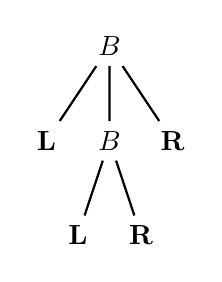
\begin{tikzpicture}[level distance=1.2cm, sibling distance=0.8cm, thick]
                            \node {$B$}
                                child {node {$\mathbf{L}$}}
                                child {node {$B$}
                                    child {node {$\mathbf{L}$}}
                                    child {node {$\mathbf{R}$}}
                                }
                                child {node {$\mathbf{R}$}};
                        \end{tikzpicture}
                        }
                        \vspace{0.2cm}\\
                        \footnotesize{
                        $0.\overline{1} \times 0.\overline{4} \approx 4.9\%$ \\
                        Likelihood
                        }
                    \end{center}
                \end{column}
                
                % Tree B
                \begin{column}{0.5\textwidth}
                    \begin{center}
                        \textbf{Correction B: \texttt{()()}}
                        \vspace{0.2cm}\\
                        \scalebox{0.75}{
                        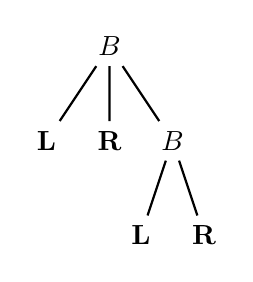
\begin{tikzpicture}[level distance=1.2cm, sibling distance=0.8cm, thick]
                            \node {$B$}
                                child {node {$\mathbf{L}$}}
                                child {node {$\mathbf{R}$}}
                                child {node {$B$}
                                    child {node {$\mathbf{L}$}}
                                    child {node {$\mathbf{R}$}}
                                };
                        \end{tikzpicture}
                        }
                        \vspace{0.2cm}\\
                        \footnotesize{
                        $0.\overline{3} \times 0.\overline{4} \approx 14.8\%$ \\
                        Likelihood
                        }
                    \end{center}
                \end{column}
            \end{columns}
        \end{column}
    \end{columns}
\end{frame}

% \begin{frame}{Future work for AXps}
%     \begin{block}{Abductive Explanations (Errors)}
%         $w = \texttt{))))}$ \\
%         \vspace{0.1cm}
%         \textcolor{blue}{\texttt{\underline{)}}}\texttt{)))},
%         \texttt{)}\textcolor{blue}{\texttt{\underline{))}}}\texttt{)}
%     \end{block}

%     \vspace{0.4cm}
    
%     % The transition block
%     \begin{center}
%     \begin{tikzpicture}[
%         box/.style={rectangle, draw=black!50, fill=yellow!10, rounded corners, thick, text width=10cm, align=center, inner sep=6pt}
%     ]
%         \node[box] {
%             \textbf{Future Work:}\\
%             If \textcolor{red}{\texttt{(}}\texttt{)}\textcolor{red}{\texttt{(}}\texttt{)} is a more common structure than \textcolor{red}{\texttt{((}}\texttt{))}.
%             We can weigh these contrastive explanations using \textbf{Probabilistic CFGs (PCFGs)}.
            
%             \textbf{The Open Question:}
%             How can we prioritize AXps?
%         };
%     \end{tikzpicture}
%     \end{center}

% \end{frame}

\begin{frame}{Future work for AXps}
    \begin{block}{Abductive Explanations (Errors)}
        $w = \texttt{))))}$ \\
        \vspace{0.1cm}
        \textcolor{blue}{\texttt{\underline{)}}}\texttt{)))},
        \texttt{)}\textcolor{blue}{\texttt{\underline{))}}}\texttt{)}
    \end{block}

    \vspace{0.4cm}
    
    % The transition block
    \begin{center}
    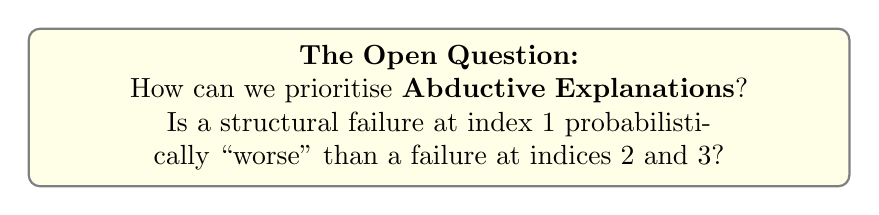
\begin{tikzpicture}[
        box/.style={rectangle, draw=black!50, fill=yellow!10, rounded corners, thick, text width=10cm, align=center, inner sep=6pt}
    ]
        \node[box] {
            \textbf{The Open Question:}\\
            How can we prioritise \textbf{Abductive Explanations}? \\
            Is a structural failure at index 1 probabilistically ``worse'' than a failure at indices 2 and 3?
        };
    \end{tikzpicture}
    \end{center}
\end{frame}


% Up to this point, we have solved explanations for deterministic systems, and we are currently using PCFGs to handle structural ambiguity. But this acts as a bridge to the ultimate goal of my research: explaining AI in dynamic, stochastic environments. >
% In the real world, like in Markov Decision Processes or reinforcement learning, actions don't have guaranteed outcomes. If an AI agent takes an action, it might succeed 80% of the time and fail 20% of the time. In these environments, an explanation can no longer be an absolute guarantee. A Contrastive Explanation must evolve into a probabilistic bound—for example, 'Changing this specific action is the minimal intervention required to raise your success rate above 95%.'

% This leaves us with exciting open questions for the final phase of my thesis: How do we extract minimal explanations over infinitely unrolling, uncertain trajectories? And how can we adapt the parsing algorithms we've built for Grammars to evaluate these dynamic behaviors?
\begin{frame}{Future Work: Explaining Stochastic Environments}
    \begin{itemize}
        \item PCFGs introduce probabilities to static sequences.
        The ultimate goal of this thesis is to scale these formalisms to explain AI in \textbf{dynamic, stochastic environments}.
    \end{itemize}

    \vspace{0.1cm}
    \begin{columns}[T]
        % LEFT COLUMN: The Environment
        \begin{column}{0.48\textwidth}
            \textbf{What is a Stochastic Environment?}\\
            \vspace{0.1cm}
            \small{Systems (like MDPs) where executing an action $a$ yields a probability distribution over future states.}\\
            \begin{center}
            \scalebox{0.75}{
            \begin{tikzpicture}[->, >=stealth, node distance=1.5cm, thick]
                \node[circle, draw, minimum size=0.8cm] (s0) {$s_0$};
                \node[circle, draw, fill=green!10, right=2cm of s0, yshift=0.8cm, minimum size=0.8cm] (s1) {$s_1$};
                \node[circle, draw, fill=red!10, right=2cm of s0, yshift=-0.8cm, minimum size=0.8cm] (s2) {$s_2$};

                \draw (s0) -- node[above, sloped, font=\footnotesize] {$a$ ($80\%$)} (s1);
                \draw (s0) -- node[below, sloped, font=\footnotesize] {$a$ ($20\%$)} (s2);
            \end{tikzpicture}
            }
            \end{center}
        \end{column}

        % RIGHT COLUMN: The Explanation
        \begin{column}{0.48\textwidth}
            \textbf{What does an explanation look like?}\\
            \vspace{0.1cm}
            \small{Explanations shift from absolute logical guarantees to probabilistic bounds.}
            
            \textbf{The Open Questions:}
            \begin{itemize}
                \item How do we define minimality for AXps/CXps when trajectories are infinite and outcomes are uncertain?
            \end{itemize}
            % \begin{block}{Stochastic CXp Example}
            %     \footnotesize{``Changing policy action $a_1$ to $a_2$ increases the probability of reaching a safe state from $40\%$ to $\geq 95\%$.''}
            % \end{block}
        \end{column}
    \end{columns}
\end{frame}



\section{Project Management}


\begin{frame}{Project Plan \& Timeline}
    
    \vspace{0.4cm}
    \begin{center}
    \scalebox{0.75}{ % Essential for keeping the chart on the slide
    \begin{ganttchart}[
        y unit title=0.5cm,
        y unit chart=0.6cm,
        x unit=0.25cm,
        vgrid={*{5}{draw=none}, dotted}, % Fixed syntax for the grid
        hgrid,
        time slot format=isodate-yearmonth,
        time slot unit=month,
        title/.append style={shape=rectangle, fill=black!10},
        title height=1,
        bar/.append style={fill=green!70!black, rounded corners=1pt}, % Darkened for projector contrast
        bar height=.6,
        bar label font=\normalsize\color{black!90},
        group top shift=.6,
        group height=.3,
        group peaks height=.2
      ]{2024-01}{2027-06}
      
      \gantttitlecalendar{year} \\
      \ganttbar{Changing Supervisors}{2024-01}{2024-05} \\
      \ganttbar{Literature Review}{2024-05}{2027-06} \\
      \ganttbar{Explaining FA}{2024-06}{2025-06} \\
      \ganttbar{Explaining CFG}{2025-03}{2026-03} \\
      \ganttbar{Explaining Stochastic Models}{2026-03}{2026-12} \\
      \ganttbar{Thesis write-up}{2027-01}{2027-06}
      
    \end{ganttchart}
    }
    \end{center}
    
    \vspace{0.4cm}
\end{frame}

\begin{frame}
    \vspace{0.6cm}
    \begin{center}
        \Large{\textbf{Thank You}}\\
        \normalsize{Questions?}
    \end{center}
\end{frame}
